\documentclass[a4paper, 12pt]{article}
\usepackage[T2A]{fontenc}
\usepackage[utf8]{inputenc}
\usepackage[english, russian]{babel}
\usepackage{graphicx}
\usepackage{amsmath}
\usepackage{listings}
\usepackage[table,xcdraw]{xcolor}

\title{Программирование на CUDA}
\author{Мураро Роман и Клюев Сергей}
\date{}

\begin{document}
\maketitle

\section{Введение}
Программирование на CUDA - это специализированная технология для параллельного программирования на графических процессорах NVIDIA. Эта технология позволяет разработчикам создавать высокопроизводительные приложения, используя графические процессоры в качестве вычислительных устройств.


\begin{figure}[!ht] 
		\centering
		
\includegraphics[scale=0.5]{kekw.png} 
		\caption{CUDA}
		\label{fig:first_image}
	\end{figure}

\section{Основные понятия}
CUDA основана на модели исполнения SIMD, где каждый поток исполнения выполняет одну и ту же инструкцию над различными данными. CUDA предоставляет программисту доступ к множеству ядер графического процессора, что позволяет эффективно распараллеливать вычисления.

\section{Требования к оборудованию и ПО}
Для работы с CUDA необходимо иметь поддерживающее её оборудование - графический процессор NVIDIA.

\section{Язык программирования и расширения}
Программирование на CUDA осуществляется на языке программирования C++. CUDA предоставляет специальные расширения языка C++, такие как специальные ключевые слова и типы данных, которые позволяют программисту использовать вычислительные возможности графического процессора.

\begin{figure}[!h] 
		\centering
		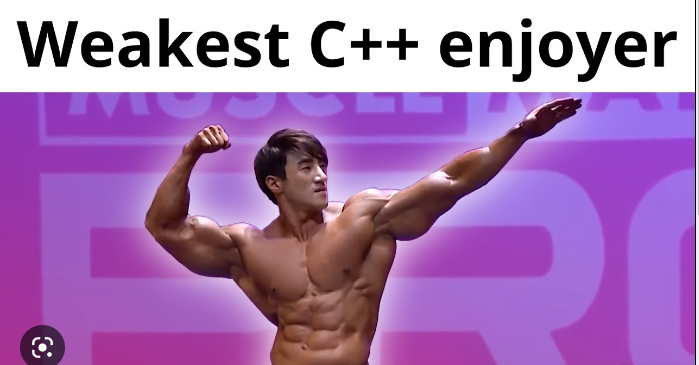
\includegraphics[scale=0.5]{cppenj.png} 
		\caption{Average C++ enjoyer}
		\label{fig:second_image}
	\end{figure}

\section{Работа с памятью}
Одной из важных частей программирования на CUDA является работа с памятью. Графические процессоры имеют свою собственную память, которая отличается от оперативной памяти компьютера. CUDA предоставляет специальные функции для выделения и копирования памяти на графический процессор, а также для доступа к этой памяти из ядер.
\begin{equation} 
		\label{eq:first_equation}
		dim3 DimGrid((N + DimBlock.x - 1)/DimBlock.x , (N + DimBlock.y -1)/DimBlock.y);
	\end{equation}
% Please add the following required packages to your document preamble:
% \usepackage[table,xcdraw]{xcolor}
% If you use beamer only pass "xcolor=table" option, i.e. \documentclass[xcolor=table]{beamer}
\begin{table}[]
\begin{tabular}{|
>{\columncolor[HTML]{FFFFFF}}c |
>{\columncolor[HTML]{FFFFFF}}c |
>{\columncolor[HTML]{FFFFFF}}c |
>{\columncolor[HTML]{FFFFFF}}c |l|}
\hline
\textit{Спецификатор} & \textit{Находится в} & \textit{Доступна для} & \textit{Вид доступа} &  \\ \hline
\_\_device\_\_        & устройстве           & устройства            & только чтение        &  \\ \hline
\_\_constant\_\_      & устройстве           & устройства и хоста    & чтение/запись        &  \\ \hline
\_\_shared\_\_        & устройстве           & блока потоков         & чтение/запись        &  \\ \hline
\end{tabular}
\end{table}

\section{Пример кода}
Ниже представлен фрагмент кода, который демонстстрирует вычисление суммы двух массивов на графическом процессоре с использованием CUDA:

\begin{lstlisting}[language=C++, basicstyle=\small]
global void add(int* a, int* b, int* c, int size) {
int i = blockIdx.x * blockDim.x + threadIdx.x;
if (i < size) {
c[i] = a[i] + b[i];
}
}

int main() {
int size = 1000;
int* a = new int[size];
int* b = new int[size];
int* c = new int[size];

int* dev_a, * dev_b, * dev_c;
cudaMalloc((void**)&dev_a, size * sizeof(int));
cudaMalloc((void**)&dev_b, size * sizeof(int));
cudaMalloc((void**)&dev_c, size * sizeof(int));

cudaMemcpy(dev_a, a, size * sizeof(int), cudaMemcpyHostToDevice);
cudaMemcpy(dev_b, b, size * sizeof(int), cudaMemcpyHostToDevice);

add<<<(size + 255) / 256, 256>>>(dev_a, dev_b, dev_c, size);

cudaMemcpy(c, dev_c, size * sizeof(int), cudaMemcpyDeviceToHost);


cudaFree(dev_a);
cudaFree(dev_b);
cudaFree(dev_c);
delete[] a;
delete[] b;
delete[] c;

return 0;
}
\end{lstlisting}

\section{Заключение}
Программирование на CUDA - это мощный инструмент для создания высокопроизводительных приложений, использующих графические процессоры. Оно требует определенных знаний и навыков, но может значительно ускорить вычисления в некоторых типах задач.





\cite{demidov2013programming}.
\cite{langdon2014genetically}.

\bibliographystyle{plain}
\bibliography{literature}

\end{document}












\end{document}